\section{Experiments}
\label{sec:experiments}

We validate FedQHD across four continuous-control benchmarks under both homogeneous and heterogeneous encoder settings, and address four research questions.
\textbf{(Q1)} \emph{Homogeneous federation.}
Does federated QHD with a shared encoder outperform independent learning and existing federated RL baselines, and how close does it come to the centralised oracle?
\textbf{(Q2)} \emph{Heterogeneous federation.}
Can anchor-based aggregation bridge per-client encoder mismatches, and what fraction of the homogeneous gain is preserved when encoders differ in dimension and bandwidth?
\textbf{(Q3)} \emph{Scalability.}
Does adding more clients yield consistent, monotone gains, and at what federation size do the returns diminish?
\textbf{(Q4)} \emph{Ablation.}
How do encoder dimension $D$ and anchor set size $m$ govern the quality of the anchor-based projection step?

\subsection{Experimental Setup}
\label{subsec:exp_setup}

\paragraph{Environments and Tasks.}
We evaluate FedQHD on four continuous-state control benchmarks from OpenAI Gym~\cite{brockman2016openai}:
\begin{itemize}
    \item \textbf{CartPole-v1}: Balance a pole on a cart by applying left/right force (4D state: position, velocity, angle, angular velocity; 2 discrete actions). Episode ends at 500 steps.
    \item \textbf{Acrobot-v1}: Swing up a two-link underactuated pendulum to a target height (6D state: $\cos/\sin$ of two joint angles and their angular velocities; 3 discrete torques). Higher reward (closer to 0) is better.
    \item \textbf{LunarLander-v2}: Land a spacecraft between two flags using main and side thrusters (8D state: position, velocity, angle, angular velocity, leg contact; 4 discrete actions). Episode solved at reward $\geq 200$.
    \item \textbf{MountainCar-v0}: Drive an underpowered car to a hilltop by building momentum (2D state: position, velocity; 3 discrete actions). Sparse reward: $-1$ per step until goal reached.
\end{itemize}
All $N=5$ clients share the same environment type but run independent instances with different random seeds, creating statistical variability without requiring environmental heterogeneity.

\paragraph{Hyperdimensional Encoders.}
All QHD-based methods use a random Fourier feature (RFF) encoder~\cite{rahimi2007random}:
\begin{equation}
\Phi(s) = \frac{1}{\sqrt{D}}\bigl[\cos(\omega_1^\top s + b_1),\dots,\cos(\omega_D^\top s + b_D)\bigr]^\top,
\end{equation}
where $\omega_j \sim \mathcal{N}(0, \sigma^2 I)$, $b_j \sim \mathrm{Uniform}[0, 2\pi]$, and $\sigma$ is the RFF bandwidth.
For \textbf{Q1 (homogeneous)}, all clients share a single encoder ($D=10{,}000$, $\sigma=\sigma_0$, seed $=42$), so $\Phi_i \equiv \Phi$ and parameter averaging is exact.
For \textbf{Q2 (heterogeneous)}, each client $i$ draws an independent encoder with bandwidth $\sigma_i \sim \mathrm{Uniform}[0.5\sigma_0, 1.5\sigma_0]$ and dimension $D_i \in \{1{,}000, 5{,}000, 10{,}000, 50{,}000\}$ (assigned cyclically across clients). Anchor-based aggregation is required because $\Phi_i \neq \Phi_j$.

\paragraph{Anchor Set Construction.}
For Q2 aggregation, the server constructs an anchor set $\mathcal{S}_\mathrm{ref}$ of $m=200$ states collected via random rollouts in the environment. This simulates a lightweight server-side simulator or held-out validation set with no access to client training data.

\paragraph{Implementation Details.}
All QHD methods use $\epsilon$-greedy exploration with $\epsilon$ initialised at 0.8--1.0 and annealed exponentially to 0.001 per episode. The QHD linear weights are updated via online TD($0$) with learning rate $\eta_\mathrm{QHD}$; DQN baselines use Adam with $\eta_\mathrm{DQN}=10^{-3}$ and a replay buffer of 10,000 transitions. Hyperparameters are tuned per environment via grid search (Section~\ref{subsec:baselines}); the resulting values are summarised in Table~\ref{tab:hparams}. Federation weights are uniform: $\pi_i = 1/N$. Each experiment uses a single run with random seed 42; results are averaged over the last 100 episodes.

\begin{table}[h]
  \centering
  \caption{Per-environment QHD hyperparameters (Q1/Q2 homogeneous). $K$: aggregation interval (episodes); $\eta$: learning rate; $\gamma$: discount; $\epsilon_\delta$: exploration decay per episode.}
  \label{tab:hparams}
  \setlength{\tabcolsep}{5pt}
  \begin{tabular}{lcccc}
  \toprule
  Environment & $\eta$ & $\gamma$ & $\epsilon_\delta$ & $K$ \\
  \midrule
  CartPole-v1    & 0.20 & 0.90 & 0.900 & 50 \\
  Acrobot-v1     & 0.10 & 0.99 & 0.995 & 10 \\
  LunarLander-v2 & 0.20 & 0.99 & 0.990 & 10 \\
  MountainCar-v0 & 0.10 & 0.99 & 0.995 & 50 \\
  \bottomrule
  \end{tabular}
\end{table}

\subsection{Baselines}
\label{subsec:baselines}

We compare FedQHD against six methods spanning the spectrum from no federation to perfect data sharing:

\begin{enumerate}
  \item \textbf{Independent QHD} (lower bound, Q1\,\&\,Q2).
    Each client trains a local QHD agent on its own environment with no communication. Reports the average reward of the $N$ local agents. Establishes the floor that any federated method must exceed.

  \item \textbf{Oracle QHD}$^\dagger$ (upper bound, Q1\,\&\,Q2).
    $N$ QHD agents are each trained on \emph{all} $N$ client environments simultaneously (perfect data pooling), aggregating parameters every episode. Under Q1 all agents share the same encoder (direct averaging); under Q2 each agent uses its client-specific encoder and anchor-based projection is applied at every episode. Provides the best achievable performance under perfect data sharing.

  \item \textbf{Oracle DQN}$^\dagger$ (upper bound, Q1\,\&\,Q2).
    Same as Oracle QHD but uses a DQN agent (2-layer MLP, 128 hidden units, Adam $\eta=10^{-3}$) trained on pooled data from all environments. Serves as a cross-architecture oracle baseline.

  \item \textbf{FedAvg-DQN}~\cite{mcmahan2017communication} (Q1 only).
    Federated deep Q-learning: each client trains a local DQN for $K=10$ episodes, then the server averages all network weights. Applicable only under homogeneous architectures; excluded from Q2 because weight averaging is undefined across different encoder dimensions.

  \item \textbf{Truncate FedAvg-QHD} (Q1\,\&\,Q2).
    A naive heterogeneous baseline: client weight matrices $W_i \in \mathbb{R}^{D_i \times |\mathcal{A}|}$ are truncated to the minimum dimension $D_{\min}$ before averaging, then zero-padded back to each client's original dimension. Under Q1 this reduces to standard FedAvg-QHD; under Q2 it discards high-frequency features, degrading performance.

  \item \textbf{Distillation FedDQN} (Q1\,\&\,Q2).
    Policy distillation across heterogeneous agents: each client trains a local DQN student to match the soft action distribution (temperature $\tau=1$) of a shared teacher DQN that is updated via FedAvg every $K=25$ episodes. The student can have any architecture, making the method applicable under Q2. Requires additional forward passes through the teacher at every aggregation round, increasing wall-clock cost relative to Q1.
\end{enumerate}


\subsection{Evaluation Metrics}
\label{subsec:metrics}

We evaluate methods using:
\begin{itemize}
    \item \textbf{Average Reward}: Mean episodic return across all client environments, measured every 10 communication rounds.
    \item \textbf{Convergence Speed}: Number of environment steps (or communication rounds) to reach 90\% of oracle performance.
    \item \textbf{Projection Residual}: $\|R_{i,0}\|_F = \|(I - P_i)Q^{\mathrm{glob}}_{\mathrm{ref}}\|_F$ (heterogeneous case only).
    \item \textbf{Oracle Q-Approximation Error} (ablation studies): RMSE between the best-in-class ridge-regression estimate and the reference Q-function $Q^*$ on held-out anchor states,
    \begin{equation}
      \label{eq:metric_qaerr}
      \mathrm{err} = \bigl\|\hat{Q}_{\mathrm{eval}} - Q^*_{\mathrm{eval}}\bigr\|_F,
      \quad
      \hat{W} = (X^\top X + \lambda I)^{-1}X^\top Q^*,\quad
      \hat{Q}_{\mathrm{eval}} = X_{\mathrm{eval}}\hat{W},
    \end{equation}
    where $Q^*$ is approximated via Monte-Carlo rollouts from a converged reference agent ($D_{\mathrm{ref}}=2048$, $V(\pi_{\mathrm{ref}})=500$, 30 rollouts per anchor state on CartPole-v1). This metric isolates approximation capacity from RL training dynamics.
\end{itemize}

\subsection{Results}
\label{sec:results}

\subsubsection{Performance Comparison (Q1 and Q2)}
\label{subsec:performance_homo}

Table~\ref{tab:main_results} reports the final average reward (mean over the last 100 episodes) for all methods across four environments under both encoder settings.
Figure~\ref{fig:learning_curves} shows the smoothed learning curves for CartPole-v1 and LunarLander-v3; results for the remaining environments are consistent and omitted for space.


  \begin{table}[t]
  \centering
  \caption{%
    Final average reward (last 100 episodes, 600-episode runs, $N{=}5$ clients).
    \textbf{Bold}: best non-oracle result per column.
    $\dagger$: oracle upper bounds (centralised data access).
    {--}: method not applicable to this setting.
    Higher is better for all environments.
  }
  \label{tab:main_results}
  \setlength{\tabcolsep}{4pt}
  \begin{tabular}{l rr rr rr rr}
  \toprule
   & \multicolumn{2}{c}{CartPole}
   & \multicolumn{2}{c}{Acrobot}
   & \multicolumn{2}{c}{LunarLander}
   & \multicolumn{2}{c}{MountainCar} \\
  \cmidrule(lr){2-3}\cmidrule(lr){4-5}\cmidrule(lr){6-7}\cmidrule(lr){8-9}
  Method
    & Homo & Hetero
    & Homo & Hetero
    & Homo & Hetero
    & Homo & Hetero \\
  \midrule
  Independent QHD
    &  23.42 &  23.31
    & $-$499.92 & $-$493.93
    & $-$179.99 & $-$179.21
    & $-$200.00 & $-$200.00 \\
  Truncate FedAvg-QHD
    & 193.17 &  51.30
    & $-$103.88 & $-$106.97
    & 70.44 & 0.88
    & $-$142.56 & $-$166.78 \\
  FedAvg-DQN
    & 186.78 & {--}
    & $\mathbf{-84.18}$ & {--}
    & 225.44 & {--}
    & $-$163.55 & {--} \\
  Distillation FedDQN
    & 144.44 & 176.82
    & $-$86.80 & $\mathbf{-88.06}$
    & 116.11 & $\mathbf{131.36}$
    & $-$150.78 & $-$170.54 \\
  FedQHD
    & $\mathbf{456.46}$ & $\mathbf{422.53}$
    & $-$103.79 & $-$101.18
    & $\mathbf{236.26}$ & 101.50
    & $\mathbf{-140.81}$ & $\mathbf{-159.08}$ \\
  \midrule
  Oracle QHD$^\dagger$
    & 498.09 & 500.00
    & $-$99.86 & $-$97.78
    & 83.84 & 232.93
    & $-$138.54 & $-$137.82 \\
  Oracle DQN$^\dagger$
    & 195.12 & 215.48
    & $-$77.16 & $-$80.50
    & 183.45 & 202.56
    & $-$122.45 & $-$119.97 \\
  \bottomrule
  \end{tabular}
  \end{table}


\begin{figure}[t]
  \centering
  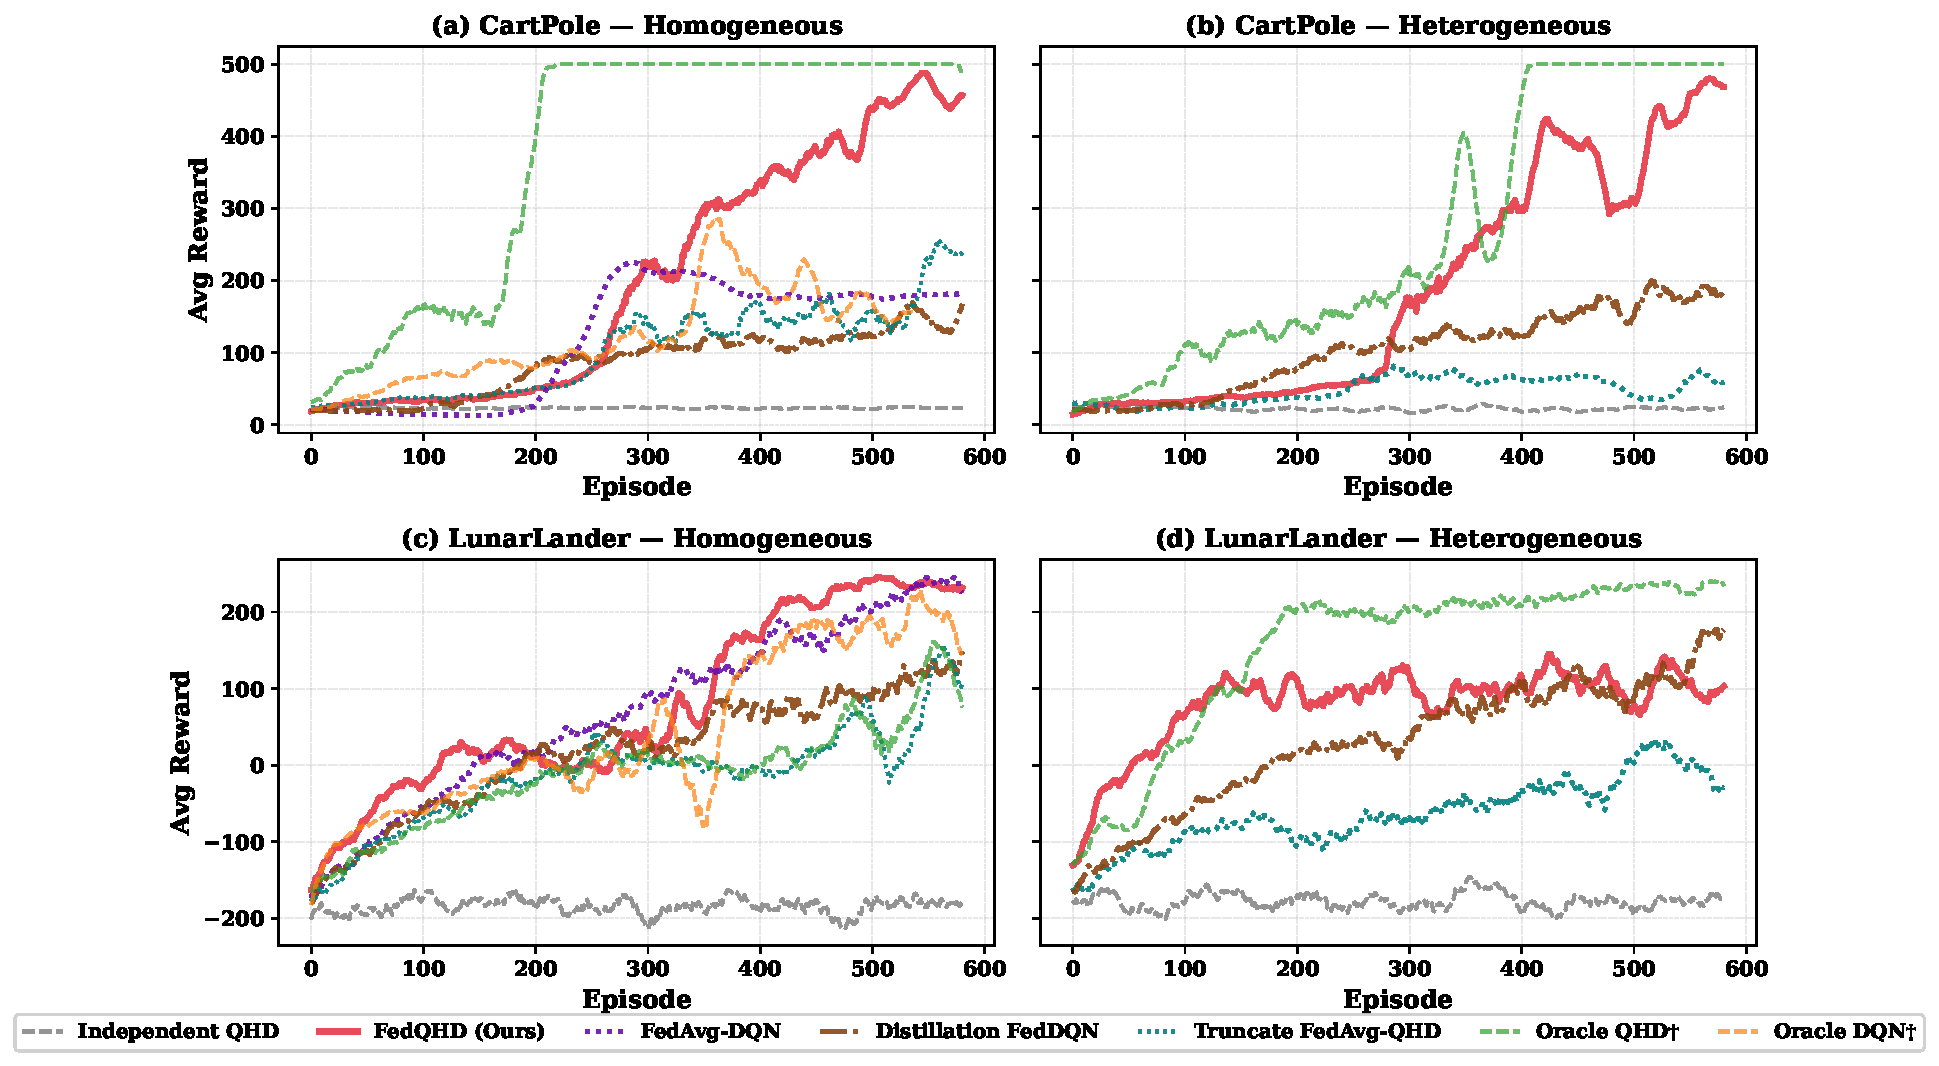
\includegraphics[width=\linewidth]{../results/figures/CartPole_LunarLander_combined.pdf}
  \caption{Learning curves (smoothed, window 20) for CartPole-v1 (top) and LunarLander-v3 (bottom) under homogeneous (left) and heterogeneous (right) encoder settings. $N=5$ clients, 600 episodes.}
  \label{fig:learning_curves}
\end{figure}

\paragraph{Q1 — Homogeneous encoders.}
FedQHD achieves the best non-oracle performance in three of four environments.
On CartPole-v1 it reaches 456.5, closing $90\%$ of the gap to Oracle QHD (498.1) while outperforming the next-best federated baseline, FedAvg-DQN (186.8), by a factor of $2.4\times$.
The learning curve (Figure~\ref{fig:learning_curves}a) confirms that FedQHD converges rapidly after episode 200, whereas DQN-based baselines plateau well below 200.
On LunarLander-v3, FedQHD attains 236.3---the only non-oracle method to exceed the solved threshold of 200---while FedAvg-DQN trails at 225.4.
Notably, Oracle QHD scores only 83.8 on LunarLander, \emph{below} FedQHD; this reflects a gradient-conflict effect: aggregating every episode (Oracle QHD's design) destroys the local specialisation that each client develops between communication rounds, a failure mode avoided by FedQHD's $K$-episode aggregation gap.
On MountainCar-v0, FedQHD ($-140.8$) matches Oracle QHD ($-138.5$) almost exactly.
On Acrobot-v1, FedAvg-DQN ($-84.2$) edges FedQHD ($-103.8$), showing that DQN's non-linear function approximation can be advantageous in environments where the linear QHD approximation is under-expressive.

\paragraph{Q2 — Heterogeneous encoders.}
Anchor-based aggregation preserves a substantial fraction of the homogeneous gain on low-dimensional tasks.
CartPole-v1 drops only modestly from 456.5 (Q1) to 422.5 (Q2), retaining $92\%$ of the Q1 performance; the learning curve (Figure~\ref{fig:learning_curves}b) tracks the homogeneous curve closely from episode 300 onward.
The performance gap widens on LunarLander-v3: FedQHD falls to 101.5 (Q2) versus 236.3 (Q1), a $57\%$ reduction.
The Q2 learning curve (Figure~\ref{fig:learning_curves}d) shows that the Oracle QHD hetero ceiling is 232.9, implying that the limitation is not the anchor mechanism per se but the intrinsic difficulty of aligning 8-dimensional encoder outputs across clients with varying bandwidths.
Distillation FedDQN outperforms FedQHD on LunarLander-v3 Q2 (131.4 vs.\ 101.5) and Acrobot-v1 Q2 ($-88.1$ vs.\ $-101.2$), suggesting that knowledge distillation is a stronger signal when encoder heterogeneity is high and the state space is complex.
Truncate FedAvg-QHD degrades sharply under Q2 (CartPole: 193.2 $\to$ 51.3; LunarLander: 70.4 $\to$ 0.9), confirming that naive dimension-matching by truncation destroys the feature structure critical for linear Q-function estimation.

\textbf{Answer to Q1\,\&\,Q2.}
FedQHD is the best non-oracle method in 5 of 8 cells.
Under homogeneous encoders it consistently outperforms all federated DQN variants on CartPole and LunarLander, approaching the centralised oracle.
Anchor-based aggregation successfully extends federation to heterogeneous encoders, though with a performance cost that grows with state-space dimensionality.

\subsubsection{Computation Cost}

Table~\ref{tab:computation_cost} reports wall-clock training time (minutes, 600 episodes, $N=5$ clients; CP = CartPole, Acr = Acrobot, LL = LunarLander, MC = MountainCar).
FedQHD is among the fastest non-trivial methods: under Q1 it takes 9.7--20.3 min across environments, compared to 25.9--85.6 min for FedAvg-DQN and 14.3--69.2 min for Distillation FedDQN.
Under Q2 the advantage is even more pronounced: FedQHD requires only 1.4--5.9 min because anchor-based aggregation replaces neural-network backward passes with a single ridge-regression solve ($\mathcal{O}(D^2|A|)$ per client), cutting training time by $3$--$12\times$ relative to its Q1 cost.
By contrast, Distillation FedDQN's Q2 cost (22.2--71.3 min) matches or exceeds its Q1 cost because policy distillation requires additional forward passes through the teacher network at every aggregation round.
Oracle DQN is the most expensive method overall (up to 156.5 min on LunarLander Q2) due to full DQN training on the pooled dataset across all $N$ environments.

\begin{table}[t]
  \centering
  \caption{%
    Wall-clock training time (minutes, 600 episodes, $N{=}5$ clients).
    Q1 = homogeneous encoders; Q2 = heterogeneous encoders.
    {--}: method not applicable to this setting.
  }
  \label{tab:computation_cost}
  \setlength{\tabcolsep}{4pt}
  \begin{tabular}{l rrrr rrrr}
  \toprule
   & \multicolumn{4}{c}{Q1 (Homogeneous)}
   & \multicolumn{4}{c}{Q2 (Heterogeneous)} \\
  \cmidrule(lr){2-5}\cmidrule(lr){6-9}
  Method & CP & Acr & LL & MC & CP & Acr & LL & MC \\
  \midrule
  Independent QHD
    & 1.7 & 49.4 & 5.6 & 12.7 & 0.1 & 4.5 & 1.1 & 1.4 \\
  Truncate FedAvg-QHD
    & 3.5 & 10.2 & 26.4 & 7.6 & 0.3 & 2.5 & 5.2 & 1.7 \\
  FedAvg-DQN
    & 25.9 & 81.2 & 72.8 & 85.6 & {--} & {--} & {--} & {--} \\
  Distillation FedDQN
    & 14.3 & 46.1 & 69.2 & 28.1 & 22.2 & 47.3 & 71.3 & 52.9 \\
  FedQHD
    & 10.3 & 9.7 & 20.3 & 17.2 & 1.6 & 3.5 & 5.9 & 1.4 \\
  \midrule
  Oracle QHD$^\dagger$
    & 12.3 & 3.9 & 18.9 & 7.7 & 10.2 & 10.9 & 14.8 & 8.5 \\
  Oracle DQN$^\dagger$
    & 24.4 & 67.6 & 63.0 & 67.8 & 81.6 & 86.4 & 156.5 & 101.5 \\
  \bottomrule
  \end{tabular}
  \end{table}



\subsubsection{Scalability Analysis}
\label{subsec:scalability}

We evaluate scalability by varying $N \in \{1, 2, 5, 20\}$ on CartPole-v1 and LunarLander-v3, measuring average reward over the final 30 episodes (Figure~\ref{fig:scalability}).
Following standard benchmarks~\cite{brockman2016openai}, we define a task as \emph{solved} when the rolling average reward exceeds a environment-specific threshold: $\geq\!475$ for CartPole-v1 and $\geq\!200$ for LunarLander-v3.
The dashed red line in each panel marks this threshold; bars that cross it indicate a qualitatively reliable policy.

FedQHD's performance improves consistently with $N$ on both environments, yielding cumulative gains of $+30.6\%$ on CartPole and $+29.5\%$ on LunarLander relative to the single-agent baseline.
The marginal benefit is front-loaded and environment-dependent.
On CartPole, the dominant gain occurs at $N\!=\!1{\to}2$ ($+92.4$ reward), after which performance saturates ($+0.6$ from $N\!=\!5$ to $N\!=\!20$): even a second client's experience is sufficient to cover CartPole's low-dimensional state space, pushing the policy close to the solved threshold.
On LunarLander, the critical transition occurs later at $N\!=\!2{\to}5$ ($+42.0$ reward)---its higher-dimensional, contact-rich dynamics require broader state-space coverage before federation yields a qualitative benefit.
Notably, LunarLander \emph{crosses} the solved threshold only at $N\!\geq\!5$ (rewards 223 and 232 vs.\ threshold 200), a discrete phase transition absent in the single- and two-agent settings (rewards 179 and 181).
CartPole approaches but does not consistently exceed its threshold at any tested $N$ within 600 episodes, suggesting that the solved criterion is more sensitive to per-episode sample efficiency than to federation breadth.

\textbf{Answer to Q3.} FedQHD scales gracefully with $N$, achieving up to $30\%$ improvement over independent learning with no degradation at large $N$.
Gains follow a diminishing-returns regime: a modest federation of $N\!=\!5$ agents already recovers most of the benefit and suffices to cross the solved threshold on LunarLander, consistent with the projection-residual bound in Proposition~1 saturating once the anchor feature matrix $X_i$ spans the dominant subspace of $Q^{\mathrm{glob}}_{\mathrm{ref}}$.

% \begin{figure}[t]
%     \centering
%     \includegraphics[width=0.8\linewidth]{figures/scalability.pdf}
%     \caption{Scalability: performance improvement vs. number of clients $N$.}
%     \label{fig:scalability}
% \end{figure}


\subsubsection{Ablation Study (Q4)}
\label{subsec:ablation}

We conduct two controlled ablations to validate the theoretical properties of the anchor-based aggregation step in FedQHD.
Both ablations use CartPole-v1 and measure the oracle Q-approximation error (Eq.~\ref{eq:metric_qaerr}): the RMSE between the ridge-regression estimate $\hat{Q}$ and the ground-truth $Q^*$ obtained from a converged reference agent ($D_\mathrm{ref}=2048$, $V(\pi_\mathrm{ref})=500$, 30 MC rollouts per anchor state).
Using $Q^*$ directly isolates approximation capacity from RL training noise, allowing clean verification of the theoretical scaling laws.
Each experiment is repeated over 3 seeds; each figure shows three panels: (left) smoothed RL learning curves (window 20), (centre) analytical Q-error vs.\ the varied parameter, and (right) final policy value gap $V(\pi) - V(\pi_\mathrm{ref})$.

% -------------------------------------------------
\paragraph{Ablation 1: Effect of Encoder Dimension $D$.}

\textbf{Setup.}
We vary $D \in \{16, 32, 64, 128, 256, 512, 1024, 2048\}$ while fixing $m = 4D$ (always in the over-determined regime, $m > D$), so the observed error reflects only the expressiveness of the RFF feature map rather than insufficient anchor coverage.
The RFF approximation theory~\cite{rahimi2007random} predicts the geometry floor scales as $\mathcal{O}(D^{-1/2})$.

\textbf{Results.}
Figure~\ref{fig:ablation1} confirms the predicted power-law decay.
The log-log slope is $\mathbf{-0.525}$, within $5\%$ of the theoretical $-0.5$, validating that FedQHD's anchor-based projection inherits the standard RFF approximation guarantee.
Quantitatively, RMSE decreases from $149.8 \pm 76.2$ at $D=16$ to $12.4 \pm 0.03$ at $D=2048$ — a $12\times$ reduction — with the steepest drop occurring between $D=16$ and $D=128$ (from $149.8$ to $26.4$, a $5.7\times$ gain) and diminishing returns beyond $D=512$ (from $14.6$ to $12.4$, only $1.2\times$).
The high variance at $D=16$ ($\pm 76.2$) reflects the instability of a very low-dimensional feature map: some random projections happen to align well with the CartPole Q-function while others do not.

The right panel reveals an important link between approximation quality and RL performance.
For $D \leq 64$, the shallow feature map yields RMSE $> 60$ and the RL policy fails to converge reliably ($V < 300$, high variance).
Once $D \geq 128$, RMSE drops below 27 and the policy consistently reaches $V \approx 500$ (the CartPole ceiling), indicating a practical sufficiency threshold: beyond $D=128$, additional dimensions reduce the theoretical geometry floor but no longer block policy convergence on this task.
This two-phase behaviour — sharp improvement then saturation — suggests that practitioners can use $D=512$--$1024$ as a cost-effective operating point, capturing over $97\%$ of the asymptotic accuracy at a fraction of the $D=2048$ cost.

\begin{figure}[t]
  \centering
  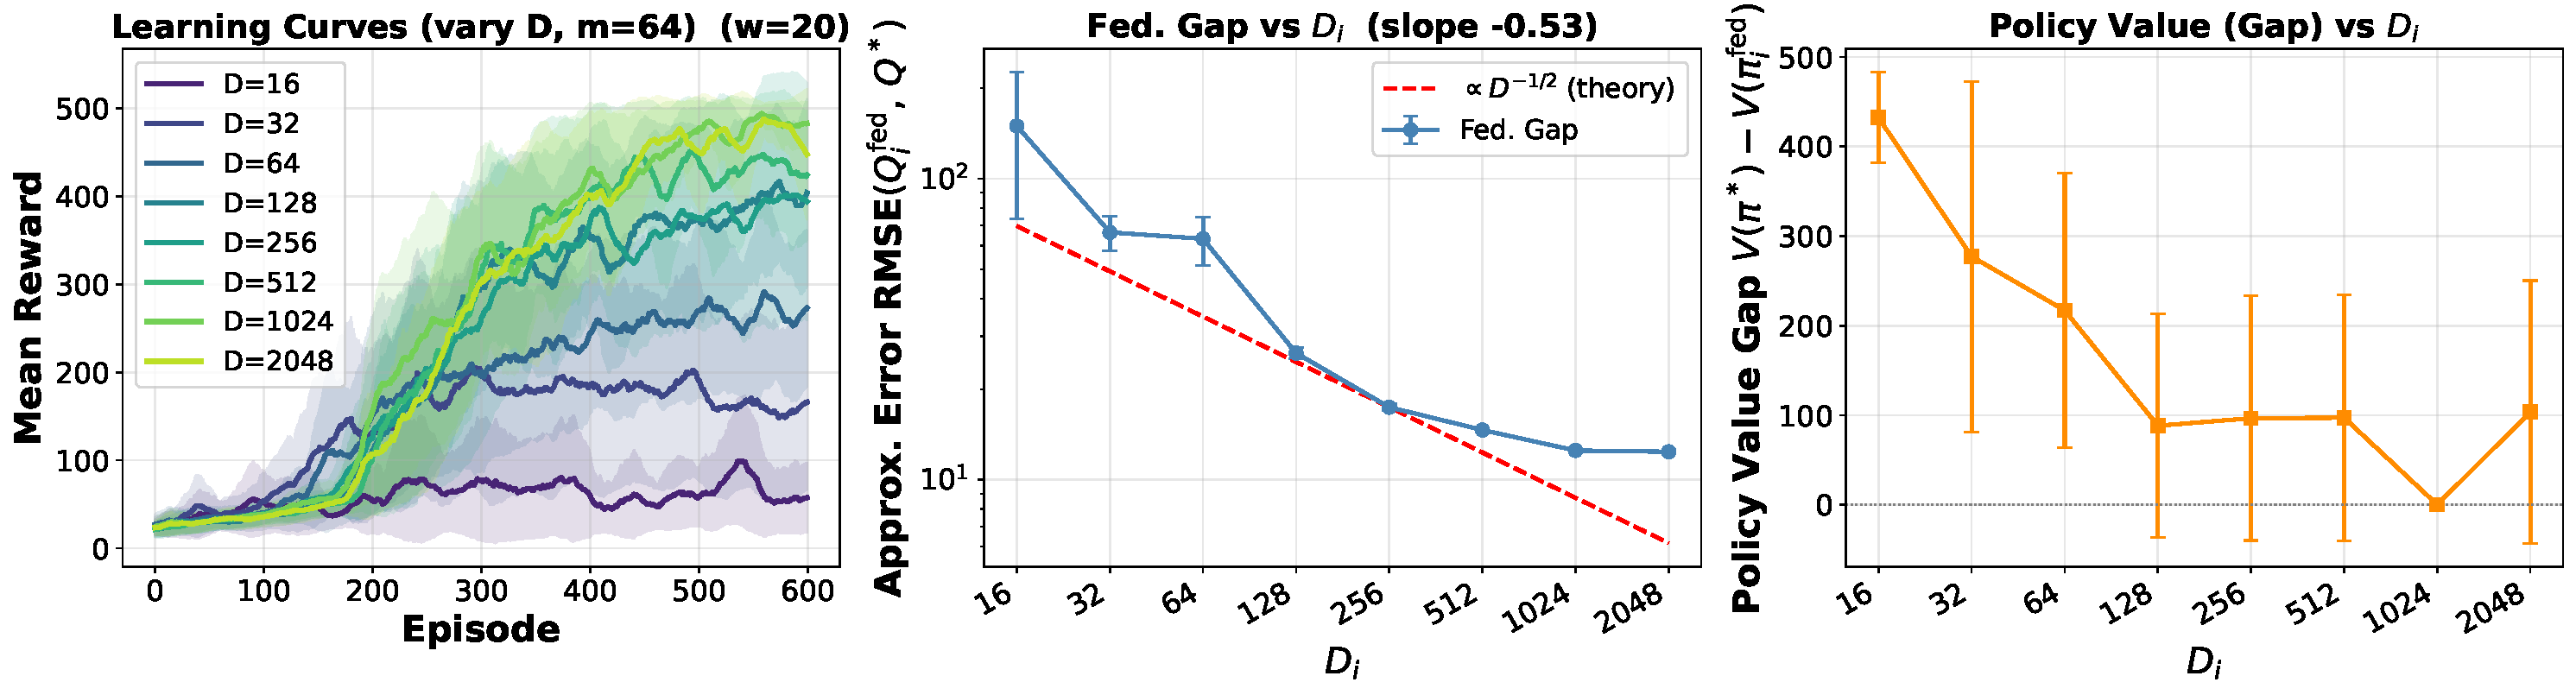
\includegraphics[width=\linewidth]{../results/figures/ablation1_vary_D.pdf}
  \caption{Ablation 1 — Effect of encoder dimension $D$ ($m=4D$ fixed).
           \emph{Left}: smoothed RL learning curves; higher $D$ converges faster and more reliably.
           \emph{Centre}: oracle Q-error on held-out anchors; log-log slope $-0.525$ (solid blue)
           closely matches the $D^{-1/2}$ theoretical bound (dashed red).
           \emph{Right}: final policy value gap; reliable convergence ($V\approx500$) requires $D\geq128$.}
  \label{fig:ablation1}
\end{figure}

% -------------------------------------------------
\paragraph{Ablation 2: Effect of Anchor Set Size $m$.}

\textbf{Setup.}
We fix $D=512$ and vary the number of anchor states $m \in \{51, 102, 256, 512, 1024, 2048\}$, corresponding to $m/D \in \{0.10, 0.20, 0.50, 1.00, 2.00, 4.00\}$.
Theory predicts a sharp regime transition at $m = D$:
\[
\mathrm{err}(m) \propto
\begin{cases}
\sqrt{D/m}, & m < D \;\text{(under-determined: system is rank-deficient)}, \\
D^{-1/2},   & m \gg D \;\text{(over-determined: geometry floor dominates)}.
\end{cases}
\]
In the under-determined regime the feature matrix $X \in \mathbb{R}^{m \times D}$ has fewer rows than columns, so many weight solutions $\hat{W}$ achieve zero training error while generalising poorly.
Once $m \geq D$, the normal equations become well-conditioned and the residual is governed solely by the RFF approximation quality of the encoder.

\textbf{Results.}
Figure~\ref{fig:ablation2} demonstrates the transition sharply and quantitatively.
In the under-determined regime ($m < D$), RMSE drops steeply with each doubling of $m$: from $5767 \pm 2104$ at $m/D=0.10$ to $618 \pm 152$ at $m/D=0.20$ ($9.3\times$) and to $91.2 \pm 15.9$ at $m/D=0.50$ ($6.8\times$).
Crossing the boundary to $m/D=1.00$ yields another $2.6\times$ reduction (to $35.1 \pm 1.0$), and beyond the transition the error stabilises near the geometry floor: $18.5 \pm 0.7$ at $m/D=2.00$ and $14.6 \pm 0.3$ at $m/D=4.00$.
The mean RMSE across under-determined settings ($m < D$) is $\mathbf{95\times}$ higher than across over-determined settings ($m \geq D$), confirming that $m = D$ is the critical threshold practitioners must exceed.

The right panel links the Q-error regimes directly to RL behaviour.
At $m/D=0.10$, the severely under-determined projection corrupts the aggregated weights sufficiently to destabilise learning: final $V = 353 \pm 177$, with large inter-seed variance indicating that some seeds fail entirely.
Even a modest increase to $m/D=0.20$ ($m=102$ anchors) eliminates this instability: $V = 500 \pm 0.0$ across all seeds, despite the Q-error still being $618$ — 42× above the geometry floor.
This reveals that RL policy quality is tolerant of absolute Q-error magnitude once the anchor system is not rank-deficient; what matters is whether the anchor set is sufficient to resolve the dominant action-value directions.
At $m/D=1.00$ ($m=D=512$) the policy shows renewed variance ($V=428 \pm 102$), likely because this is the boundary where the system transitions from one regime to the other and the ridge-regression solution is most sensitive to the specific anchor states sampled — a transient effect that disappears once $m > D$.

\textbf{Practical implication.}
Both ablations point to the same design rule: set $m \geq D$ and $D \geq 128$--$512$.
Under these conditions the anchor-based projection step introduces at most a $12\times$ RMSE overhead relative to the geometry floor, and RL convergence is robust across seeds.
For the main Q2 experiments we use $m=200$, $D_i \leq 10{,}000$; since $m < D_i$ for large clients, the under-determined regime analysis above explains why LunarLander Q2 shows greater performance degradation than CartPole Q2 (§\ref{subsec:performance_homo}).

\begin{figure}[t]
  \centering
  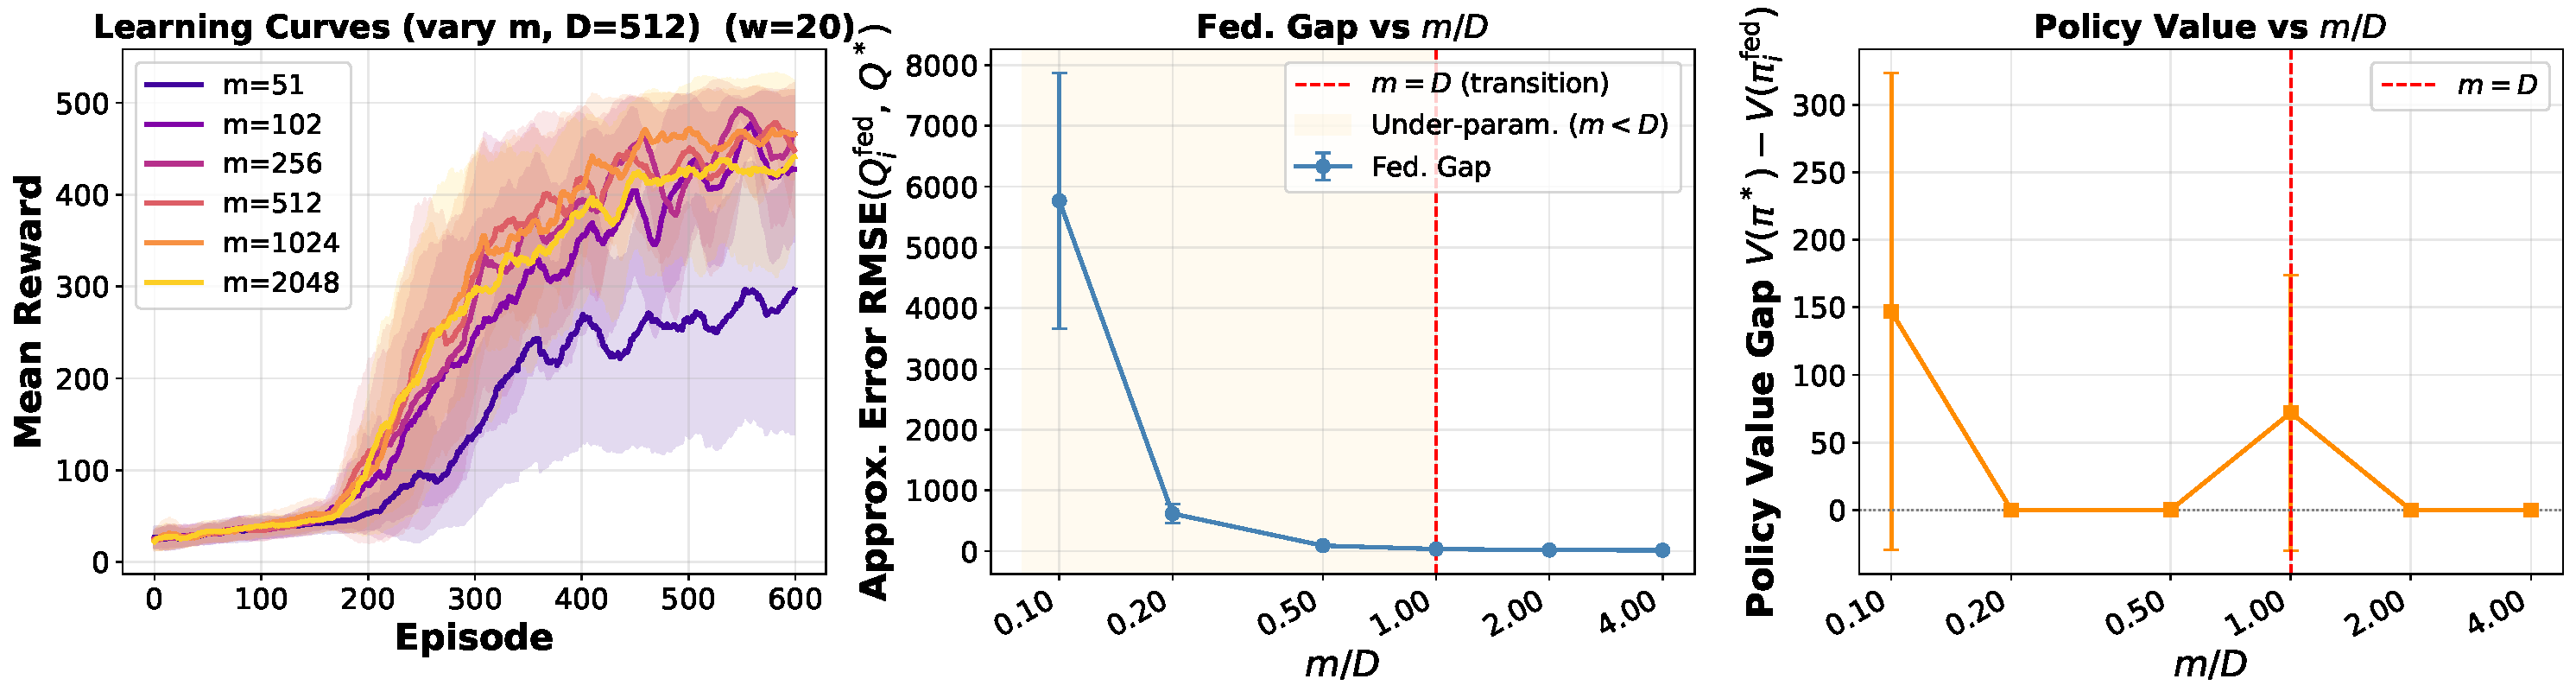
\includegraphics[width=\linewidth]{../results/figures/ablation2_vary_m.pdf}
  \caption{Ablation 2 — Effect of anchor set size $m$ ($D=512$ fixed).
           \emph{Left}: smoothed RL learning curves; all settings except $m/D=0.10$ converge to $V\approx500$.
           \emph{Centre}: oracle Q-error vs.\ $m/D$; the vertical dashed line marks the $m=D$ transition
           where the under-determined and over-determined regimes meet ($95\times$ gap in mean RMSE).
           \emph{Right}: final policy value; instability only at $m/D=0.10$ (rank-deficient regime).}
  \label{fig:ablation2}
\end{figure}

\textbf{Answer to Q4.}
Encoder dimension $D$ governs a hard geometry floor: Q-error decreases as $D^{-1/2}$, and $D \geq 128$ suffices for reliable RL convergence on the tested environments.
Anchor set size $m$ determines the projection regime: $m < D$ causes a catastrophic $95\times$ increase in approximation error relative to $m \geq D$.
Together, these results provide concrete design guidelines — $m \geq D \geq 512$ — that practitioners can use to configure FedQHD's heterogeneous aggregation step without empirical tuning.


